% multivolume e-book
\documentclass[oneside,12pt]{book}
\usepackage[paperwidth=210mm,paperheight=148mm,margin=10mm]{geometry}
% \usepackage{xr}

% Cyrillization
\usepackage[T1,T2A]{fontenc}
\usepackage[utf8]{inputenc}
\usepackage[english,russian]{babel}
\usepackage{indentfirst}

% pdflatex options
\usepackage{hyperref}
\newcommand{\email}[1]{$<$\href{mailto:#1}{#1}$>$}
\usepackage[pdftex]{graphicx}
% \usepackage[unicode,colorlinks,linkcolor=blue,bookmarks=true]{hyperref}
% \usepackage[usenames,dvipsnames,svgnames]
\usepackage[usenames,svgnames]{xcolor}

% font setup for screen reading
\renewcommand{\familydefault}{\sfdefault}
\normalfont

% relative sectioning
\usepackage{ifthen}
\newcounter{secdepth}\setcounter{secdepth}{0}
\newcommand{\secup}{\addtocounter{secdepth}{1}}
\newcommand{\secdown}{\addtocounter{secdepth}{-1}}
\newcommand{\secrel}[1]{
\ifthenelse{\equal{\value{secdepth}}{0}}{\part{#1}}{}
\ifthenelse{\equal{\value{secdepth}}{-1}}{\chapter{#1}}{}
\ifthenelse{\equal{\value{secdepth}}{-2}}{\section{#1}}{}
\ifthenelse{\equal{\value{secdepth}}{-3}}{\subsection{#1}}{}
\ifthenelse{\equal{\value{secdepth}}{-4}}{\subsubsection{#1}}{}
}

% extra char sets
\usepackage{wasysym} % smileys
\usepackage{amssymb} % windows key

% listings
\usepackage{verbatim}
\usepackage{listings}
\lstset{
basicstyle=\small, % or \tiny \small or \footnotesize
extendedchars=true,inputencoding=utf8, % i18n
frame=single, % show frames around
numbers=left, numberstyle=\small,numbersep=1mm,% line numbering
tabsize=4, % tab style
keywordstyle=\color{Blue},%\texttt,
keywordstyle={[2]\color{Green}},%\texttt,
keywordstyle={[3]\color{Magenta}},%\texttt,
keywordstyle={[4]\color{Red}},%\texttt,
keywordstyle={[5]\color{Blue}},%\texttt,
commentstyle=\color{Cyan}%\texttt%,
% showspaces=false
}

\usepackage{lstmk}\lstdefinestyle{mk}{language=mk}
\usepackage{lstrc}\lstdefinestyle{rc}{language=rc}
\usepackage{lstsyslinux}\lstdefinestyle{syslinux}{language=syslinux}

\newcommand{\lst}[3]{\lstinputlisting[title=\href{#2}{#1}]{#3}}
\newcommand{\lstx}[4]{\lstinputlisting[title=\href{#2}{#1},language=#4]{#3}}

% software menu & keys
\usepackage[os=win]{menukeys}
\newcommand{\winstart}{$\boxplus$}
% \newcommand{\winr}{\keys{\winstart+R}}
% \newcommand{\file}[1]{\textbf{\textsf{#1}}}
% \newcommand{\lms}{$\lhd$}
% \newcommand{\dblms}{$\lhd\lhd$}
% \newcommand{\rms}{$\rhd$}
\newcommand{\checkbox}{$\boxtimes$}
\newcommand{\uncheckbox}{$\square$}

% misc
\usepackage{framed}

\newcommand{\note}[1]{\footnote{\ #1}}
\newcommand{\cp}[1]{\note{копипаста: #1}}
\newcommand{\term}[1]{\emph{#1}}
\newcommand{\prog}[1]{\textcolor{Brown}{#1}}
\newcommand{\pack}[1]{\textcolor{Green}{#1}}
\newcommand{\file}[1]{\textbf{#1}}
\newcommand{\internet}{Internet}
\newcommand{\cpp}{$C^{+}_{+}$}
\newcommand{\py}{Python}

\newcommand{\cm}[1]{Cortex-M#1}
\newcommand{\cmx}{\cm{x}}

\newcommand{\odina}{1А616}

\newcommand{\linux}{Linux}
\newcommand{\win}{\winstart Windows}
\newcommand{\make}{make}

\newcommand{\ram}{ОЗУ}


% % % \documentclass[oneside,12pt]{book}
% % % 
% % % % e-book format
% % % \usepackage[paperwidth=210mm,paperheight=148mm,margin=10mm]{geometry}
% % % 
% % % % Cyrillization
% % % \usepackage[T1,T2A]{fontenc}
% % % \usepackage[utf8]{inputenc}
% % % \usepackage[english,russian]{babel}
% % % \usepackage{indentfirst}
% % % \usepackage{enumitem} 
% % % 
% % % % font setup for screen reading
% % % \renewcommand{\familydefault}{\sfdefault}
% % % \normalfont
% % % 
% % % % pdflatex options
% % % \usepackage[unicode,colorlinks,linkcolor=blue,bookmarks=true]{hyperref}
% % % \usepackage[pdftex]{graphicx}
% % % \usepackage[usenames,dvipsnames,svgnames]{xcolor}
% % % 
% % % % relative sectioning
% % % \usepackage{ifthen}
% % % \newcounter{secdepth}\setcounter{secdepth}{0}
% % % \newcommand{\secup}{\addtocounter{secdepth}{1}}
% % % \newcommand{\secdown}{\addtocounter{secdepth}{-1}}
% % % \newcommand{\secrel}[1]{
% % % \ifthenelse{\equal{\value{secdepth}}{0}}{\part{#1}}{}
% % % \ifthenelse{\equal{\value{secdepth}}{-1}}{\chapter{#1}}{}
% % % \ifthenelse{\equal{\value{secdepth}}{-2}}{\section{#1}}{}
% % % }
% % % 
% % % % listings
% % % \usepackage{verbatim}
% % % \usepackage{listings}
% % % \lstset{
% % % basicstyle=\small, % or \tiny \small or \footnotesize
% % % extendedchars=true,inputencoding=utf8, % i18n
% % % frame=single, % show frames around
% % % numbers=left, numberstyle=\small,numbersep=1mm,% line numbering
% % % tabsize=4, % tab style
% % % keywordstyle=\color{Blue},%\texttt,
% % % keywordstyle={[2]\color{Green}},%\texttt,
% % % keywordstyle={[3]\color{Magenta}},%\texttt,
% % % keywordstyle={[4]\color{Red}},%\texttt,
% % % keywordstyle={[5]\color{Blue}},%\texttt,
% % % commentstyle=\color{Cyan}%\texttt%,
% % % % showspaces=false
% % % }
% % % 
% % % \usepackage{lstmk}\lstdefinestyle{mk}{language=mk}
% % % \usepackage{lstrc}\lstdefinestyle{rc}{language=rc}
% % % \usepackage{lstsyslinux}\lstdefinestyle{syslinux}{language=syslinux}
% % % 
% % % \newcommand{\lst}[3]{\lstinputlisting[title=\href{#2}{#1}]{#3}}
% % % \newcommand{\lstx}[4]{\lstinputlisting[title=\href{#2}{#1},language=#4]{#3}}
% % % 
% % % % software menu & keys
% % % \usepackage[os=win]{menukeys} 
% % % \usepackage{amssymb} % windows key
% % % \newcommand{\winstart}{$\boxplus$}
% % % \newcommand{\winr}{\keys{\winstart+R}}
% % % \newcommand{\file}[1]{\textbf{\textsf{#1}}}
% % % \newcommand{\lms}{$\lhd$}
% % % \newcommand{\dblms}{$\lhd\lhd$}
% % % \newcommand{\rms}{$\rhd$}
% % % \newcommand{\checkbox}{$\boxtimes$}
% % % \newcommand{\uncheckbox}{$\square$}
% % % 
% % % % disable oneliner page breaks
% % % \usepackage[defaultlines=2,all]{nowidow}
% % % 
% % % % books bib management
% % % \usepackage{biblatex}
% % % \addbibresource{../bib/python.bib}
% % % \addbibresource{../bib/eskd.bib}
% % % \addbibresource{../bib/electronics.bib}
% % % \addbibresource{../bib/latex.bib}
% % % \addbibresource{../bib/sat.bib}
% % % \addbibresource{../bib/math.bib}
% % % \addbibresource{../bib/sysdesign.bib}
% % % 
% % % \usepackage{makeidx}
% % % \makeindex
% % % 
% % % % extra char sets
% % % \usepackage{wasysym} % smileys
% % % 
% % % % set lists style
% % % \usepackage{enumitem}
% % % \setlist{nosep}
% % % 
% % % % misc
% % % 
% % % % \usepackage{titling}
% % % 
% % % \newcommand{\email}[1]{$<$\href{mailto:#1}{#1}$>$}
% % % \newcommand{\internet}{Internet}
% % % 
% % % \newcommand{\cm}[1]{Cortex-M#1}
% % % \newcommand{\cmx}{\cm{x}}
% % % 
% % % \newcommand{\linux}{Linux}
% % % \newcommand{\emlinux}{em\linux}
% % % 
% % % \newcommand{\cpp}{$C^{+}_{+}$}
% % % \newcommand{\py}{Python}
% % % 
% % % \newcommand{\vcs}{\hyperref[vcs]{VCS}}
% % % \newcommand{\make}{\hyperref[make]{Make}}
% % % \newcommand{\spice}{ngSPICE}
% % % \newcommand{\latex}{\LaTeX}
% % % 
% % % \newcommand{\eclipse}{\textcircled{$\equiv$}\textsc{eclipse}}
% % % \newcommand{\vim}{(g)Vim}
% % % 
% % % \newcommand{\note}[1]{\footnote{\ #1}}
% % % \newcommand{\cp}[1]{\note{копипаста \url{#1}}}
% % % 
% % % \newcommand{\win}{\winstart Windows}
% % % 
% % % \newcommand{\mk}{МК}
% % % 
% % % \newcommand{\ram}{RAM}
% % % 
% % % 
% % % \newcommand{\pref}[1]{/стр.\pageref{#1}/}
% % % 
% % % % icon sets
% % % \newcommand{\icoesch}{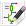
\includegraphics[height=0.1\textheight]{tmp/icon_eeschema.png}}
% % % % selecting
% % % \usepackage{framed}
% % % \newcommand{\term}[1]{\textcolor{Green}{#1}}
% % % \renewcommand{\emph}[1]{\textcolor{Blue}{#1}}
% % % \newcommand{\prog}[1]{\textcolor{Brown}{#1}}
% % % \newcommand{\pack}[1]{\textcolor{Magenta}{#1}}
% % % 
% % % \newcommand{\odina}{1А616}
% % % 
% % % % math
% % % \usepackage{cancel}
% % % 
% % % % titles
% % % 
% % % \hypersetup{
% % % 	pdftitle={Азбука халтурщика-ARMатурщика},
% % % 	pdfauthor={ruOpenWrt, HackSpace <<Чебураторный завод>>, Консорциум хоббитов
% % % 	России, Bill Collis (Часть 1)}, 
% % % 	pdfsubject={https://github.com/ponyatov/Azbuka}
% % % % }
